\documentclass[12pt,a4paper]{article}
\usepackage{fullpage}
\pagestyle{plain}
\usepackage{amsmath}
\usepackage{graphicx}
\usepackage{indentfirst}
\graphicspath{{./img}}
% choose any of the following packages to support AmsTeX
%\usepackage{amsmath,amssymb,amsfonts,mathrsfs,mathptm,bm,mathtools}
% choose the following package to insert eps figures
% for png, jpg or pdf figures, use pdflatex
%\usepackage{graphicx}

\newcommand{\question}[1]{\bigskip\noindent{\textbf{Q{#1} solution}}}

% set HW number
\newcommand{\HWnum}{2}
% specify first and last name and the ID number of students in the group
% append asterix to indicate who is making the submission
\newcommand{\StudentA}{Hanggang Zhu$^\ast$, 3200110457}
\newcommand{\StudentB}{Suhao Wang, 3200110777}
\newcommand{\StudentC}{Lumeng Xu 3200110184}

% ===============================================================
\begin{document}

%%% header
{\noindent \rule{\linewidth}{0.2mm}}\\
\noindent{ECE 374, ZJUI, Spring 2023\hfill%
  \textbf{\large H{}W\HWnum\ Solutions} \hfill \today\smallskip}

\noindent{\hfill \StudentA, \StudentB, and \StudentC \hfill}
\\[-0.2cm]{\noindent \rule{\linewidth}{0.2mm}}
%%% end header



\question{4.A}

\question{4.B}

\question{4.C}

\question{4.D}

\question{4.E}

\question{4.F}

Strings not containing subsequence $000$ is equivalent to having at most two $0$s. The regular expression simply consider three cases.
Solution: $1^* + 1^*01^* + 1^*01^*01^*$

\question{4.G}

The string can also be interpreted as string whose substring with no $11$s come before substring with no $00$s.String with no $11$:$(\epsilon + 1)(0(\epsilon + 1 ))^*$. String with no $00$: $(\epsilon + 0)(1(\epsilon + 0))^*$.Concatenate them and simply.
Solution: $(\epsilon + 1)(0(\epsilon + 1))^*(1(\epsilon + 0))^*$


\question{4.H}

Strings not containing subsequence $010$ means that $1$ can't be in the middle of two $0$s. So $1$ must be on one side of $0$s.
Solution: $1^*0^*1^*$

\question{4.I}

Given four continuous $0$s, we can't put $1$s between every cut of these $0$s. If we remove these $1$s, we can get $0^*1^*0^*1^*0^*$(remove one $1$s) or $0^*1^*0^*$(remove two $1$s) and $0^*$(remove three $1$s). They are all included in the case of $0^*1^*0^*1^*0^*$. We generalize it by adding $1$s at two sides.
Solution:$1^*0^*1^*0^*1^*0^*1^*$

\question{4.J}

Strings not containing subsequence $10$ means $0$s must come before $1$s.
Solution:$0^*1^*$


\question{5.A}
\\The DFA is drawn below.
\\The DFA accepts all strings that contain an even number of 0s and an even number of 1s.
Each state records the number of 0s or 1s so far.
\\  \hspace*{1em} \textbf{Formal Description:}
\\ \begin{center}
$Q=\{q0EE,q1EO,q2OO,q3OE\}$, 
\\where the front letter represents whether the number of 0 is even or not, and the later number
represents whether the number of 1 is even or not.
\\ $s=q0$
\\ $A=\{q0\}$
\\ $\delta\{q0,0\}=q3$
\\ $\delta\{q0,1\}=q1$
\\ $\delta\{q1,0\}=q2$
\\ $\delta\{q1,1\}=q0$
\\ $\delta\{q2,0\}=q1$
\\ $\delta\{q2,1\}=q3$
\\ $\delta\{q3,0\}=q0$
\\ $\delta\{q3,1\}=q2$
\end{center}
Each state is unique, and $q0$ is the start state and the accepting 
state, no matter how many number of 0s or 1s are read, the machine
can only be accepted when returning to $q0$.

\newpage

\begin{figure}
  \centering
  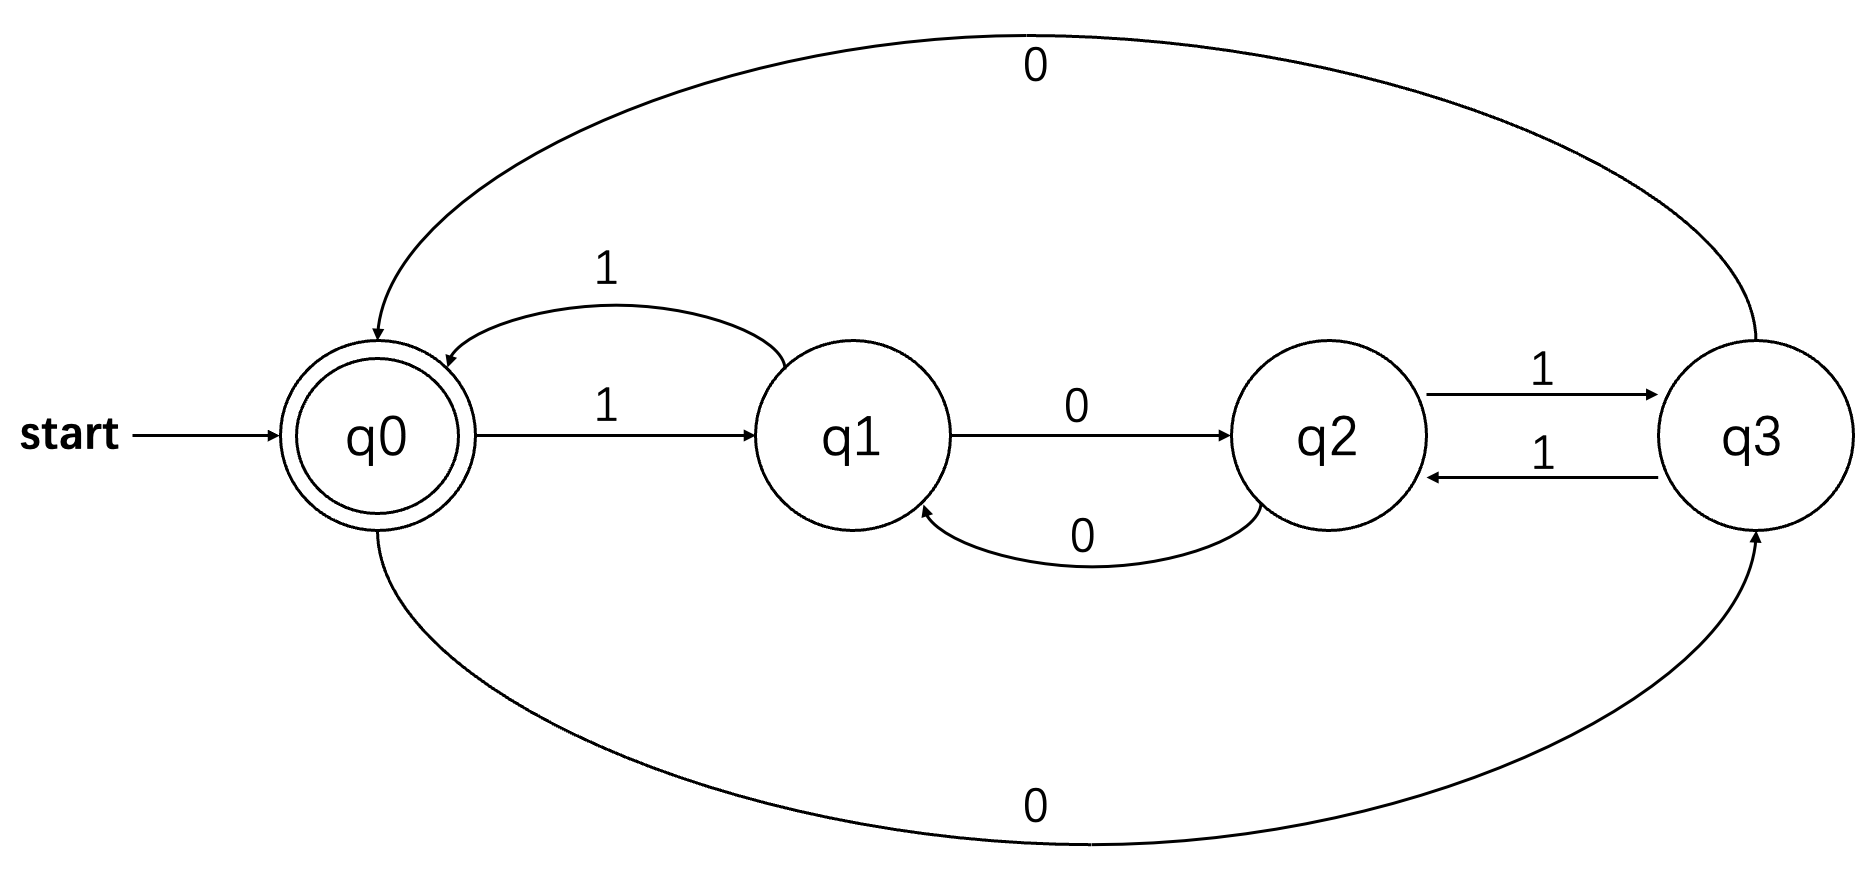
\includegraphics[width = 0.7\textwidth]{img/374hw2.png}
\end{figure}

\question{5.B}
\\According to the state removal method, 
\\if $q1=\delta(q0,x)$ and $q2=\delta(q1,y)$, then $q2=\delta(q1,y)=
\delta(\delta(q0,x),y)=\delta(q0,xy)$
\\After removing the states $q1$ and $q2$, we get the following image:
\begin{figure}
  \centering
  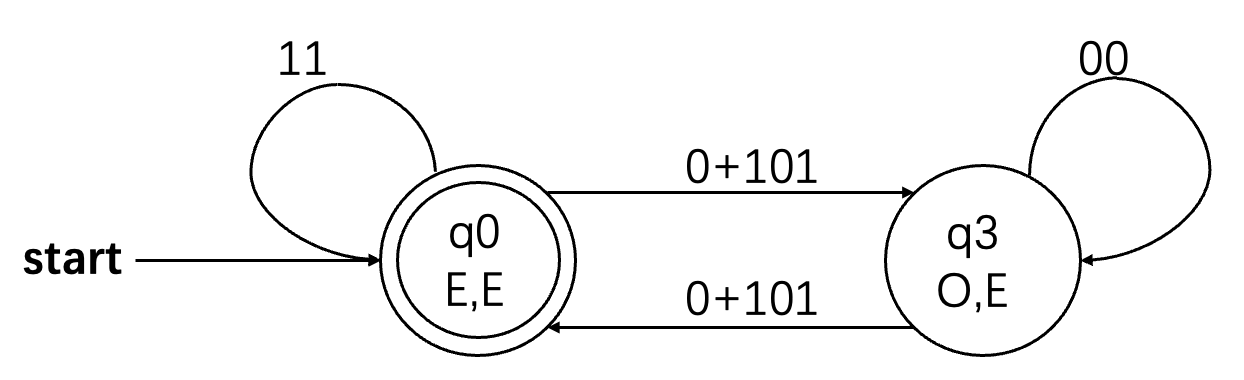
\includegraphics[width = 0.6\textwidth]{img/hw2_2.png}
\end{figure}
\\So,we get the regular expression for the simplified machine : $11+(0+101)(00)^\ast (0+101)$.
\\Then, after further simplifying, we get the graph below:
\begin{figure}
  \centering
  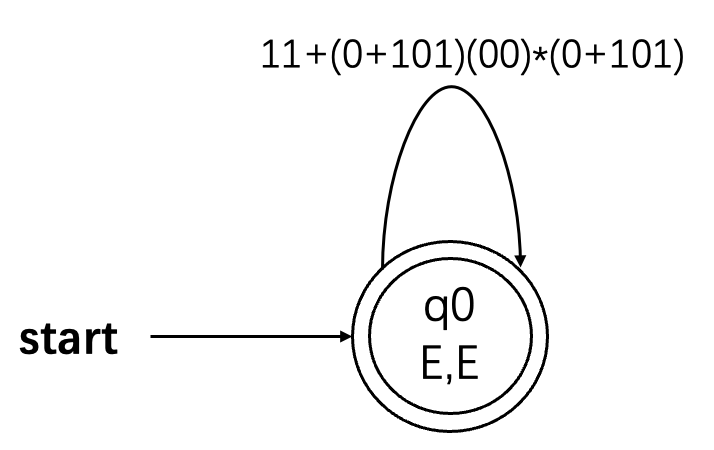
\includegraphics[width = 0.6\textwidth]{img/hw2_3.png}
\end{figure}
\\So, we get the regular expression of L is $(11+(0+101)(00)^\ast (0+101))^\ast$.
\\Then, for the argument that this expression is correct, first, we consider the strings
do not contain any consecutive 0s or 1s, that is, the input is the empty string. According 
to this expression, it is just the accepting state, which satisfies the condition.
\\What's more, from the regular expression, we can see that it only accepts even number of 0s
and even number of 1s, other kinds of numbers are not allowed. So, this expression is correct.

\question{6.A}

\noindent For language $L = L_1 \cap L_2 \cap L_3$, formally describe the DFM as  $M = (Q,\sum,\delta,s,A)$, where

$\bullet$ $Q = Q_1 \times Q_2 \times Q_3 = \{(q_1,q_2,q_3)\ \vline\ q_1 \in Q_1, q_2 \in Q_2, q_3 \in Q_3\}$

$\bullet$ $\delta:Q \times \sum \rightarrow Q \mbox{ ,where } \delta((q_1,q_2,q_3),a) = (\delta_1(q_1,a),\delta_2(q_2,a),\delta_3(q_3,a)) \mbox{ and } a \in \sum$

$\bullet$ $s = (s_1,s_2,s_3)$

$\bullet$ $A = A_1 \times A_2 \times A_3 = \{(q_1,q_2,q_3)\ \vline\ q_1 \in A_1, q_2 \in A_2, q_3 \in A_3\}$

\question{6.B}

For $\delta^*(q,w)$, we have the formal definition:

\begin{equation*}
\delta^*(q,w) = 
  \begin{cases}
    q & \mbox{, if } w = \epsilon, \\
    \delta^*(\delta(q,a),x) & \mbox{, if } w = ax
  \end{cases}
\end{equation*}

Now we prove by induction. 

$\bullet$ \textbf{Base case:} Let $w$ be an artibrary string of length 0. we get $w = \epsilon$. Then
\begin{align*}
\delta^*((q_1,q_2,q_3),w) &= \delta^*((q_1,q_2,q_3),\epsilon) \\
    &= (q_1,q_2,q_3) \\ 
    &= (\delta_1^*(q_1,\epsilon), \delta_2^*(q_2,\epsilon), \delta_3^*(q_3,\epsilon)) \\
    &= (\delta_1^*(q_1,w), \delta_2^*(q_2,w), \delta_3^*(q_3,w))
\end{align*}

$\bullet$ \textbf{Induction hypothesis:} For any string $w$ of length $n > 0$, we have that
\begin{equation*}
  \delta^*((q_1,q_2,q_3),w) = (\delta_1^*(q_1,w), \delta_2^*(q_2,w), \delta_3^*(q_3,w))
\end{equation*}

$\bullet$ \textbf{Inductive step:} Let $w$ be an artibrary string with length $n > 0$. Assume inductive hypothesis holds for all strings x of length $< n$. Then we have $w = ax$ for some string x with length $< n$ and $a \in \sum$. We have:
\begin{align*}
  \delta^*((q_1,q_2,q_3),w) &= \delta^*(\delta((q_1,q_2,q_3), a), x) &\mbox{(definition of $\delta^*(q,w)$) }\\
      &= \delta^*((\delta_1(q_1,a), \delta_2(q_2,a), \delta_3(q_3,a)), x) &\mbox{(definition of $\delta$ in Q6.A)}\\
      &= (\delta_1^*(\delta_1(q_1,a), x),\delta_2^*(\delta_2(q_2,a), x),\delta_3^*(\delta_3(q_3,a), x)) &\mbox{(induction hypothesis)}\\
      &= (\delta_1^*(q_1,w), \delta_2^*(q_2,w), \delta_3^*(q_3,w)) &\mbox{(definition of $\delta^*(q,w)$) }
\end{align*}

So, the equation is proved.


\question{6.C}

\question{6.D}


\end{document}

